\documentclass[10pt,letterpaper]{article}

% Packages
\usepackage[utf8]{inputenc}
\usepackage[top=0.85in,left=1.5in,footskip=0.75in]{geometry}
\usepackage{lastpage,fancyhdr,graphicx}
\usepackage{epstopdf}
\usepackage{verbatim}
\usepackage{amsmath}
\usepackage{amsfonts}
\usepackage{hyperref}
\usepackage{setspace}

% Text layout
\raggedright
\setlength{\parindent}{0.5cm}
\textwidth 5.5in 
\textheight 8.75in
\onehalfspacing

% Bibliography
\usepackage[backend=biber,style=numeric,sorting=ynt]{biblatex}
\addbibresource{bibliography.bib}

% C++ symbol
\newcommand{\CC}{C\nolinebreak\hspace{-.05em}\raisebox{.4ex}{\tiny\bf +}\nolinebreak\hspace{-.10em}\raisebox{.4ex}{\tiny\bf +}}
\def\CC{{C\nolinebreak[4]\hspace{-.05em}\raisebox{.4ex}{\tiny\bf ++}}}

% Header and footer
\pagestyle{fancy}
\fancyhf{}
\rfoot{\thepage/\pageref{LastPage}}
\renewcommand{\headrulewidth}{0pt}
\fancyheadoffset[L]{2.25in}
\fancyfootoffset[L]{2.25in}

\begin{document}

\vspace*{0.2in}

\begin{centering}
{\Huge\textbf\newline{Pandemia: User Guide}}
\\
\bigskip

\includegraphics[width=0.2\textwidth]{pandemia_logo}
\\
\bigskip
\today
\\
\end{centering}

\tableofcontents

\section{Introduction}

Pandemia is an individual-based stochastic pandemic simulator. It if able to simulate and visualize the spread of an infectious disease across multiple geographical regions. These regions could represent the countries of the world, or the administrative divisions of a single country. The model is fast and scalable, able to simulate extremely large numbers of individuals, while supporting a wide range of highly adaptable features.

This software can be used by researchers looking to assess the impact of policy in the context of a public health emergency caused by an infectious disease of humans. The disease could, for example, be a respiratory infectious disease spread by a coronavirus or an influenza virus.

The emergence and re-emergence of infectious diseases threatens the health and well-being of people all over the world, and tools such as Pandemia can play a vital role in supporting pandemic preparedness and response.

This user guide presents an introduction to the software and its various components.

- parallel processing
- scale factor
- random seed

\section{World}

The Pandemia simulator acts upon a \textbf{World}. A \textbf{World} consists of \textbf{Regions}, with each \textbf{Region} consisting of \textbf{Agents}, \textbf{Locations} and \textbf{Activities}. Each agent performs a sequence of activities, and performs these activities in particular locations. A \textbf{World} additionally consists of a \textbf{Travel Matrix}, representing how many agents travel from each region to each other region each day. Here is the simplest possible \textbf{World} structure:
\begin{itemize}
\item One \textbf{Region}, one \textbf{Activity}, one \textbf{Location} and any number of \textbf{Agents}.
\end{itemize}
Here is the most complicated:
\begin{itemize}
\item Several \textbf{Regions}, with each \textbf{Region} consisting of several \textbf{Activities}, any number of \textbf{Locations} and any number of \textbf{Agents}, with a \textbf{Travel Matrix} describing the mixing between regions.
\end{itemize}

\subsection{Agents}
An individual human being is referred to as an \textbf{Agent}. Each agent is described by their age, a weekly routine of activities, locations at which the agent might perform these activities, and weights indicating the probabilities of these locations being chosen.

\subsection{Locations}
A \textbf{Location} represents, for example, an area of land or a building, such as a house, restaurant, shop or school classroom. A location is described by its type, and a pair of spatial coordinates.

\subsection{Activities}
An \textbf{Activity} is something an agent does, for example cooking, driving to work, or shopping. Activities are simply labels, with no deeper structure.

\subsection{Regions}
A \textbf{Region} represents, for example, a country or administrative division. A region consists of a set of activities, a set of agents, and a set of locations.

\subsection{World Factory}
A World is built by a \textbf{World Factory}. Different worlds are built either by changing the configuration of a world factory, or by using a different world factory entirely.

\subsection{Vectorization}
Once a \textbf{World} has been built, it is then converted into a \textbf{Vector World}. This is done by converting each \textbf{Region} into a \textbf{Vector Region}. A \textbf{Vector Region} is a vectorized version of a \textbf{Region}, in which data is formatted as arrays of integers and floats, as opposed to Python lists and dictionaries. This facilitates interface with libraries of functions written in C.

\section{Simulator}

The model features of a number of components, most of which are optional:
\begin{itemize}
\item \textbf{Movement}
\item \textbf{Travel}
\item \textbf{Health}
\item \textbf{Hospitalization}
\item \textbf{Testing and Contact Tracing}
\item \textbf{Vaccination}
\item \textbf{Seasonality}
\end{itemize}
Additional or alternative components are easily added. Pandemia provides a default model for each component. The details of these default models are described in separate documents. The main Pandemia loop looks approximately as follows:
\begin{center}
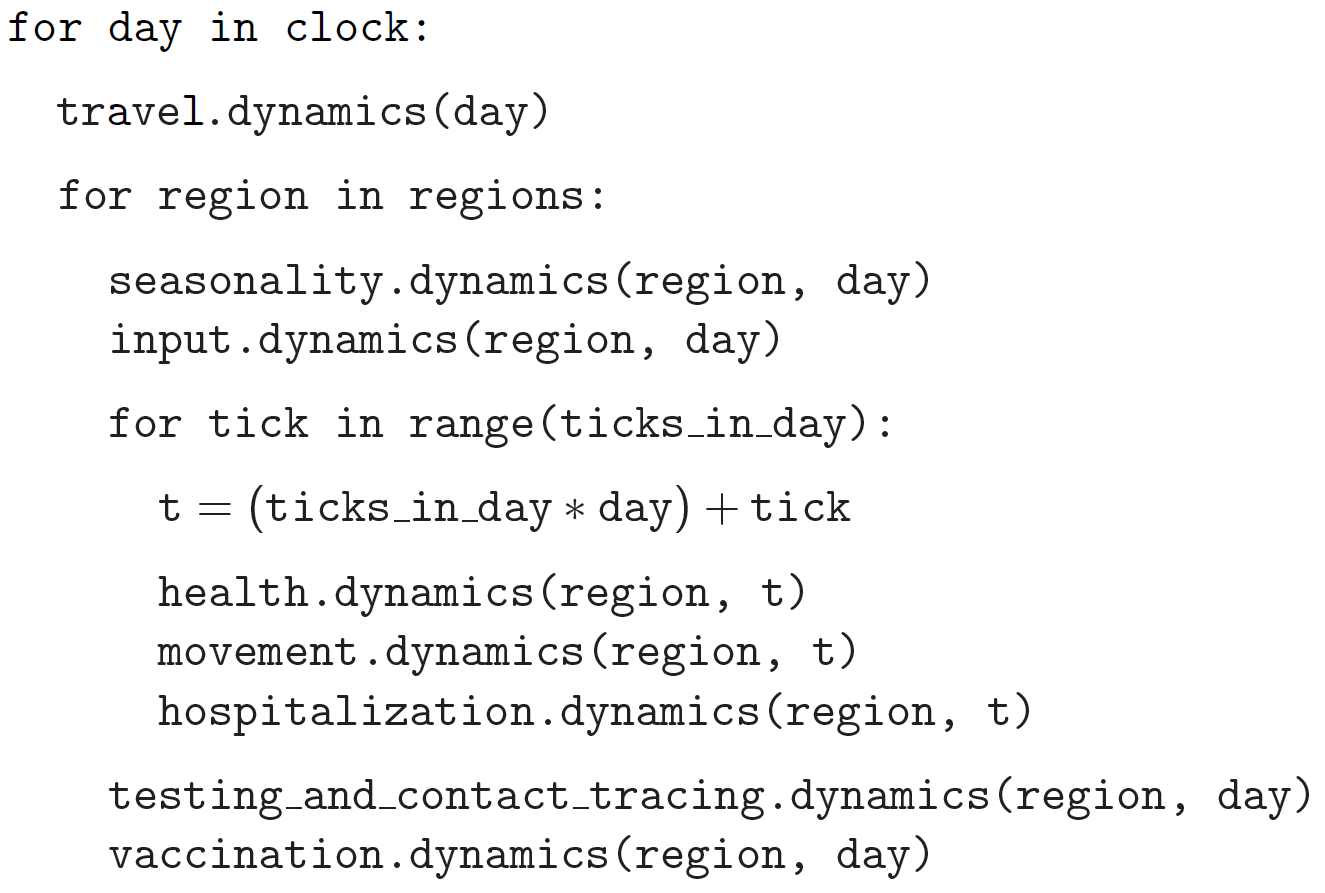
\includegraphics[width=0.65\textwidth]{psuedo}
\end{center}
Note that some components update each day, while others update each tick. At the beginning of each day, Pandemia decides who is travelling from each region to each other region, and infects these travellers based on the average infectiousness of their destination region. These travellers are then set aside for the remainder of the day. Pandemia then loops over all the regions, performing independent individual-based simulations on a finer timescale. Since these simulations are independent, the loop over the regions can be parallelized. In this way, Pandemia is both fast and scalable. Even on a laptop computer, using 15 CPUs and 24GB of RAM, it has been able to perform a 100 day simulation, with a 1 hour tick length, of over 100 million individuals, in under 1.5 hours.


The \textbf{Input} component allows the user to specify a \textbf{Policy}, consisting of interventions. Possible interventions include the following:
\begin{itemize}
\item \textbf{Lockdown}
\item \textbf{Border Closure}
\item \textbf{Vaccination}
\item \textbf{Testing and Contact Tracing}
\item \textbf{Quarantine}
\item \textbf{Face Masks}
\end{itemize}
Additional or alternative interventions are easily added. \textbf{Reporters} collect output data for visualization and analysis.


The \textbf{World} object, having been built, can be saved and thus it is not necessary to complete the build phase each time a simulation is run. The \textbf{World} object is fed into the simulator.

\subsection{Clock}

\subsection{World}

\subsection{Components}

\subsection{Simulator Factory}

\subsection{Reporters}

\section{Movement}

The Pandemia model acts on a \textbf{World}, with each \textbf{World} consisting of \textbf{Regions}, with each \textbf{Region} consisting of \textbf{Individuals}, \textbf{Locations} and \textbf{Activities}. Each individual performs a sequence of activities and performs these activities at particular locations. During the building of the \textbf{World}, each individual is assigned a weekly routine, starting on a Sunday, consisting of a sequence of activities.

For example, suppose in a given region there are three activities, \textbf{Home}, \textbf{Work} and \textbf{School}, and that tick length is set equal to 8 hours, meaning that there are 3 ticks of the simulation clock per day. Then a possible weekly routine could be:
\begin{center}
[\textbf{Home}, \textbf{Home}, \textbf{Home}, \textbf{Home}, \textbf{Work}, \textbf{Home}, \textbf{Home}, \textbf{Work}, \textbf{Home}, \textbf{Home}, \textbf{Work}, \textbf{Home}, \textbf{Home}, \textbf{Work}, \textbf{Home}, \textbf{Home}, \textbf{Work}, \textbf{Home}, \textbf{Home}, \textbf{Home}, \textbf{Home}]
\end{center}
representing a typical working week, or alternatively 
\begin{center}
[\textbf{Home}, \textbf{Home}, \textbf{Home}, \textbf{Home}, \textbf{School}, \textbf{Home}, \textbf{Home}, \textbf{School}, \textbf{Home}, \textbf{Home}, \textbf{School}, \textbf{Home}, \textbf{Home}, \textbf{School}, \textbf{Home}, \textbf{Home}, \textbf{School}, \textbf{Home}, \textbf{Home}, \textbf{Home}, \textbf{Home}]
\end{center}
representing a typical school week.

During the building of the \textbf{World}, each individual is assigned a weighted set of locations for each activity. These are the locations at which an individual can perform each activity. During the simulation, whenever an individual switches from one activity to another, the individual randomly selects a new location from the set of allowed locations, according to the weights.

For example, suppose in a given region there are two activities, \textbf{Home} and \textbf{Other}. Then, a given individual might be assigned a single location for the activity \textbf{Home}, with weight $1.0$, and several other locations for the activity \textbf{Other}, with weights chosen according to the distance of each location from the home, so that locations further from home are less likely to be visited, and so on.

Upon changing activity, individuals may also put on or take off a face mask, depending on the activity and the current policy on face masks.

If the change of location is prohibited by policy interventions, then the individual is directed to their home location. In particular, each individual must for the default movement model be assigned a home location.

\section{Travel}

\section{Health}
Epidemic models typically represent health using discrete states. In a typical compartmental model, the population is partitioned into subsets, labelled \textit{Susceptible}, \textit{Infected}, \textit{Recovered} and \textit{Dead}. These compartments can then be subdivided, and new compartments added, to produce increasingly complicated models.

This approach runs into difficulties once partial immunity is introduced, since the compartmental label \textit{Recovered} then becomes ambiguous. It runs into further difficulties once multiple strains of the pathogen are introduced, since then the label \textit{Susceptible} becomes ambiguous.

Pandemia therefore dispenses with the compartmental framework altogether, taking an entirely new approach to modelling individual health. In Pandemia, the health of an individual is described by five attributes:
\begin{itemize}
\item \textbf{Strain}
\item \textbf{Disease}
\item \textbf{Infectiousness}
\item \textbf{Immunity (outer layer)}
\item \textbf{Immunity (inner layers)}
\end{itemize}
The immune system is represented using layers, with the outer layer determining whether or not an infection is blocked, and the inner layers determining the outcome for infections that are not blocked. A key innovation of Pandemia is that, for each individual, these five attributes are stored as \textit{functions}.

\subsection*{Variables}
The value of an attribute at time $\texttt{t}$ is given by evaluating the corresponding function at time $\texttt{t}$. During a simulation, the following variables store the values of these functions at the current time:
\begin{itemize}
\item \texttt{current{\_}strain}
\item \texttt{current{\_}disease}
\item \texttt{current{\_}infectiousness}
\item \texttt{current{\_}sigma{\_}immunity{\_}failure}
\item \texttt{current{\_}rho{\_}immunity{\_}failure}
\end{itemize}
The prefix \texttt{sigma{\_}} refers to the outer layer, while the prefix \texttt{rho{\_}} refers to the inner layers.

\subsection*{\texttt{current{\_}strain}}
For individual $\texttt{n}$, the variable $$\texttt{current{\_}strain[n]}$$ indicates whether or not individual $\texttt{n}$ is infected, and if so with which strain. The variable is an integer, taking values in the range $$\texttt{\{-1, 0, 1, 2, \ldots, S - 1\}}$$ where $\texttt{S}$ denotes the number of strains. If the individual is not infected, then $$\texttt{current{\_}strain[n] = -1}.$$ We assume that individuals can only be infected with one strain at a time.

\subsection*{\texttt{current{\_}disease}}
For individual $\texttt{n}$, the variable $$\texttt{current{\_}disease[n]}$$ indicates the extent to which individual $\texttt{n}$ is diseased. The variable is a float, taking values in the range $\texttt{[0,1]}.$ If the individual has no disease, then $$\texttt{current{\_}disease[n] = 0}.$$ If the individual is dead, then $$\texttt{current{\_}disease[n] = 1}.$$ Values close to $\texttt{1}$ represent severe illness, values close to $\texttt{0}$ represent mild illness. Values above a threshold represent symptomatic illness, values below the threshold represent asymptomatic illness. 

\subsection*{\texttt{current{\_}infectiousness}}
For individual $\texttt{n}$, the variable $$\texttt{current{\_}infectiousness[n]}$$ indicates the extent to which individual $\texttt{n}$ is infectious. The variable is a float, taking non-negative values. If the individual is infected but not infectious, then $$\texttt{current{\_}infectiousness[n]} = 0.$$ If the individual is infected, then increasing the value of this variable increases the probability that the individual transmits strain $\texttt{current{\_}strain[n]}$ to other individuals.

\subsection*{\texttt{current{\_}sigma{\_}immunity{\_}failure}}
For individual $\texttt{n}$ and strain $\texttt{s}$, the variable $$\texttt{current{\_}sigma{\_}immunity{\_}failure[n][s]}$$ represents the probability that the immune system of individual $\texttt{n}$ \textit{fails} to prevent an infection when confronted with strain $\texttt{s}$. Being a probability, this variable is therefore a float taking values in the range $\texttt{[0,1]}.$ Since this variable stores a failure probability, values closer to $\texttt{0}$ represent higher levels of protection.

\subsection*{\texttt{current{\_}rho{\_}immunity{\_}failure}}
If an infection has occurred, then sigma immunity has failed and the pathogen has made it past the outer layer of defence. It now confronts a number of internal layers. Each layer has a probability of failing to stop the pathogen, with the outcome of the infection getting progressively worse the deeper the pathogen penetrates. This binary tree structure allows the user to parametrize, for example, the efficacy of a vaccine against symptomatic illness, severe illness and death. If the pathogen passes through all but the last internal layer, which is impenetrable, then the individual experiences the worst possible outcome.

For example, suppose the model is configured in such a way that there are two internal layers. Then, for a given individual, infected with a given strain, there are two possible outcomes. If the first internal layer fails to stop the pathogen, the outcome will be the latter of the two outcomes. If the first internal layer is successful, then the outcome will be the former of the two outcomes. These two outcomes could, for example, be configured to represent mild and severe illness.

More generally, suppose the model is configured in such a way that there are $\texttt{R}$ internal layers (and therefore $\texttt{R}$ possible outcomes). Then, for individual $\texttt{n}$ and strain $\texttt{s}$, the variable $$\texttt{current{\_}rho{\_}immunity{\_}failure[n][s]}$$ gives an array of probabilities, of length $\texttt{R}$, corresponding to the \textit{failure} probabilities of each layer. If a pathogen makes it past layer $\texttt{r}$, then it moves on to face layer $\texttt{r+1}$, else the individual gets outcome $\texttt{r}$. Since the last layer is impenetrable, the final entry in this array is always set equal to $\texttt{0}$, meaning that the last layer never fails to stop the pathogen. This procedure is completed immediately after infection.

While sigma immunity determines whether or not an infection occurs, with rho immunity determining the outcome of that infection, to understand the outcomes themselves we must discuss the $\texttt{health{\_}presets}$.

\subsection*{Presets and Updates}

Pandemia determines the default response to an infection for each individual, for each strain, in advance of the simulation. In particular, if an individual has been assigned the preset response $\texttt{p}$, from the set of possible preset responses $\texttt{health{\_}presets}$, then the object $\texttt{p[r]}$ contains parameters which determine updates for each of the five health attributes described above, corresponding to outcome $\texttt{r}$.

For example, suppose that our model features two strains and two internal layers. Then the object $\texttt{p[r]}$ may look as follows:
\begin{center}
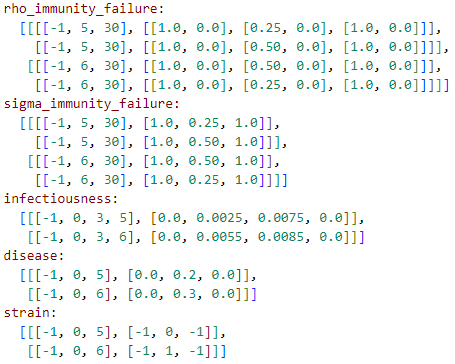
\includegraphics[width=0.5\textwidth]{codeexample}
\end{center}
The numbers in these arrays encode step functions. For example, the pair of arrays $\texttt{[[-1,0,5], [0.0,0.2,0.0]]}$ encodes the step function $f$ given by
\begin{equation}
f(t) =
\begin{cases}
0.0 \text{ for } t < 0 \\
0.2 \text{ for } 5 > t \geq 0 \\
0.0 \text{ for } t \geq 5
\end{cases}.
\end{equation}

Suppose in the example that individual $\texttt{n}$ has just been infected with strain $\texttt{0}$, and that the infection has resulted in outcome $\texttt{r}$, with $\texttt{p[r]}$ as above. Then the variable $\texttt{current{\_}strain[n]}$ will take the value $\texttt{0}$ for the next $\texttt{5}$ days, at which time it returns to the value $\texttt{-1}$, indicating that the individual is no longer infected. The variable $\texttt{current{\_}disease[n]}$ will take the value $\texttt{0.2}$ for the next $\texttt{5}$ days, at which time it returns to the value $\texttt{0.0}$, indicating that the individual has recovered. The variable $\texttt{current{\_}infectiousness[n]}$ will take the value $\texttt{0.0025}$ for the next $\texttt{3}$ days, followed by $\texttt{0.0075}$ for $\texttt{2}$ days, after which time it returns to the value $\texttt{0.0}$, indicating that the individual is no longer infectious.

Updates to the sigma and rho immunity variables are more complicated. The immunity variables are updated via the operation of function multiplication. Recall that the immunity functions store probabilities of failure, so the product of such functions give the probabilities of failure for overlapping immune responses, assuming independence.

Suppose in the above example that individual $\texttt{n}$ has no immunity against either strain prior to infection. Assume that the infection with strain $\texttt{0}$ occurred at time $\texttt{t}$. Then, after updating their immunity functions, the component of their sigma immunity function corresponding to strain $\texttt{0}$ will be given by the step function $$\texttt{[-1, t + 5, t + 30], [1.0, 0.25, 1.0]},$$ while the component corresponding to strain $\texttt{1}$ will be given by $$\texttt{[-1, t + 5, t + 30], [1.0, 0.5, 1.0]}.$$

In particular, for 25 days following the end of their infection, the probability that their immune system fails to protect against another infection by strain $\texttt{0}$ is improved from $\texttt{1.0}$ to $\texttt{0.25}$, after which it returns to $\texttt{1.0}$, representing a loss of immunity. The probability that their immune system fails to protect against an infection by strain $\texttt{0}$ is improved from $\texttt{1.0}$ to $\texttt{0.5}$, after which it returns to $\texttt{1.0}$, representing a loss of cross immunity.

Suppose now that at time $\texttt{t + 10}$ individual $\texttt{n}$ is again infected by strain $\texttt{0}$. Then between times $\texttt{t + 10}$ and $\texttt{t + 15}$, the three variables describing their current strain, disease and infectiousness will be updated as before. But the component of their sigma immunity function corresponding to strain $\texttt{0}$ will now be subject to appropriate multiplication, after which it will be given by the step function $$\texttt{[-1, t + 5, t + 15, t + 30, t + 40]},$$ $$\texttt{[1.0, 0.25, 0.0625, 0.25, 1.0]}.$$ In particular, between times $\texttt{t + 15}$ and $\texttt{t + 30}$ there are overlapping immunity responses, so that in order for a third infection to occur by strain $\texttt{0}$, the pathogen must overcome the immune response generated by the first infection \textit{and} the immune response generated by the second infection. Our assumption is that these events are independent, hence the multiplication of probabilities.

Updates to rho immunity are similar, except that these functions are now array-valued, these arrays corresponding to the failure probabilities for each internal layer, so the functions must be multiplied component-wise.

For a preset $\texttt{p}$ and outcome $\texttt{r}$, while the components of $\texttt{p[r]}$ corresponding to strain, disease and infectiousness are vectors, each containing precisely $\texttt{S}$ functions, where $\texttt{S}$ is the number of strains, the components corresponding to rho and sigma immunity are matrices, containing precisely $\texttt{S} \times \texttt{S}$ functions, the additional dimension accounting for possibility of cross-immunity, as in the above example.

\subsection*{Transmission}

For a location $l$ in region $i$, we define:
\begin{equation*}
p_l := \left(1 - \prod_{m \in l} (1 - f_m)\right)
\end{equation*}
where $m \in l$ means all individuals $m$ currently in location $l$, with
\begin{equation*}
f_m  := \omega_m \nu_m \mu(i) \lambda(l) \beta(s_m).
\end{equation*}
Here
\begin{itemize}
\item $\omega_m$ is the current face mask multiplier associated to individual $m$, which takes the value $1$ if they are not wearing a face mask, and some number smaller that $1$ if they are;
\item $\nu_m$ is the current infectiousness of individual $m$;
\item $\mu$ is a multiplier depending on the region $i$, reflecting for example seasonal changes in transmission that act on the regional level;
\item $\lambda$ is a multiplier depending on the location $l$, reflecting the fact that some types of location might be less conducive to transmission than others;
\item $\beta$ is a control coefficient depending on the strain $s_m$ that individual $m$ is currently infected with, if any.
\end{itemize}
For each susceptible individual $n$ in location $l$, with current face mask multiplier $\omega_n$, the probability that they are exposed at this time is then assumed to be $\omega_n p_l$. If such an individual is exposed, then to determine which strain they are exposed to, we assume the expression
\begin{equation*}
\frac{\sum_{\{m \in l: s_m = s\}} f_m}{\sum_{\{m \in l\}} f_m}
\end{equation*}
gives the probability that they are exposed to strain $s$. Given this exposure, the probability that they are actually infected with strain $s$ is then $\sigma_{ns}$, the current sigma immunity of individual $n$ against strain $s$. The outcome of this infection is then determined by the rho immunity of the individual, according the procedure outlined in the previous subsections.

\subsection*{SIR Rescaling}

If the option $\texttt{sir{\_}rescaling}$ is set to $\texttt{True}$, then the transmission probabilities are rescaled in such a way that approximates the homogeneous mixing of standard compartmental models. Moreover, this option allows for the activation of a mixing matrix, that can be used to describe mixing between population subgroups, for example age groups.

For example, suppose we have only one region, one location, one strain and no face masks. Suppose that $\nu_m = 1$ if $m$ is infected, with $\nu_m = 0$ otherwise. Denote by $N_{a}$ the number of people in group $a$ and by $h$ the step size. Then the rescaling factor for the transmission probabilities becomes $h / N_a$. In particular, denoting by $m_{ab}$ the mixing between groups $a$ and $b$ and by $I_b$ the number of currently infected individuals in age group $b$, for an individual $n$ in group $a(n)$, we have:
\begin{align} \nonumber
p_n =\, & 1 - \prod_{b} \left(1 - \frac{h \beta m_{a(n) b}}{N_b}\right)^{I_b} \\ \nonumber
\approx\, & 1 - \prod_{b \in A} \exp \left(-\frac{h\beta m_{a(n)b} I_b}{N_b}\right)\\ \nonumber
 = \, & 1 - \exp \left(- \sum_{b} \frac{h\beta m_{a(n)b} I_b}{N_b}\right)\\[2mm] \nonumber
 = \, & 1 - \exp \left(- h\beta (MI)_{a(n)}\right) \nonumber
\end{align}
where $M_{ab} := m_{ab} / N_b$ is the normalized mixing matrix. This is consistent with a standard compartmental model, since the expected number of new infections in age group $a$ at time $t$ then satisfies the approximation
\begin{align} \nonumber
\mathbb{E}\left[\frac{S_a(t+h) - S_a(t)}{h}\right] \approx\, & -S_a(t)\left(\frac{1 - \exp \left(- h\beta (MI(t))_{a}\right)}{h}\right)\\[2mm] \nonumber
\approx\, & -\beta S_a(t) (MI(t))_a. \nonumber
\end{align}
In particular, with only one population subgroup we have $M = 1 / N$, therefore recovering the first equation
\begin{equation*}
\frac{d}{dt} S(t) = - \beta \frac{S(t)I(t)}{N}
\end{equation*}
of the SIR model. With exponentially distributed recovery times, and no reinfection, we recover the remaining equations, and therefore arrive at a stochastic approximation of the SIR model.

With the option $\texttt{sir{\_}rescaling}$ set to $\texttt{True}$, the default health model is therefore a stochastic individual-based generalization of the SIR model. On the other hand, with the option $\texttt{sir{\_}rescaling}$ set to $\texttt{False}$, the transmission probabilities are not divided by the number of individuals in each location, meaning that adding susceptible individuals to the location of an infected individual does not dilute the infectiousness of that individual, as it does under the SIR rescaling. For example, if Alice and Bob are riding a bus, and Bob is infectious, then under the SIR rescaling the probability that Alice is infected by Bob decreases if more susceptible people get on the bus. This may not be realistic, so by default the rescaling is set to $\texttt{False}$.

\section{Hospitalization}

\section{Testing and Contact Tracing}

\section{Vaccination}

\section{Seasonality}

\section{Input}

\section{Optimization}

\end{document}